% Gabarit pandoc des corrigés publiés (brut et guidé). Contenu sans marque ni nom de site.
% Compilation : lualatex (latexmk -lualatex).
% Le Markdown reste la source unique : ne pas éditer ce fichier .tex à la main.
\documentclass[11pt,a4paper]{article}

% --- Moteur, polices (Latin Modern) et langue ---------------------------------
\usepackage{iftex}
\ifLuaTeX\else\errmessage{Ce document se compile avec lualatex}\fi
\usepackage{amsmath,amssymb,mathtools}
\usepackage{fontspec}
% mathrm=sym : \mathrm prend ses glyphes dans la police mathématique (ℓ, μ, Ω), comme KaTeX.
\usepackage[math-style=TeX,bold-style=TeX,mathrm=sym]{unicode-math}
% Repli pour les glyphes absents de Latin Modern (indices et exposants Unicode,
% flèches, filets des schémas en texte, symboles) : DejaVu, puis Latin Modern Math
% (ℓ, lettres mathématiques Unicode des légendes).
\directlua{
  luaotfload.add_fallback("repliTexte", {"DejaVuSerif:mode=harf;", "DejaVuSans:mode=harf;", "file:latinmodern-math.otf:mode=harf;"})
  luaotfload.add_fallback("repliMono", {"DejaVuSansMono:mode=harf;", "DejaVuSans:mode=harf;", "file:latinmodern-math.otf:mode=harf;"})
}
\setmainfont{Latin Modern Roman}[RawFeature={fallback=repliTexte}]
\setsansfont{Latin Modern Sans}[RawFeature={fallback=repliTexte}]
\setmonofont{Latin Modern Mono}[RawFeature={fallback=repliMono}]
\setmathfont{Latin Modern Math}
\usepackage[french]{babel}
\frenchsetup{SmallCapsFigTabCaptions=false}

% --- Mise en page --------------------------------------------------------------
\usepackage[a4paper,margin=2.2cm,headheight=14pt,footskip=1.2cm]{geometry}
\usepackage{microtype}
\setlength{\emergencystretch}{4em}
\tolerance=1500
\setlength{\parindent}{0pt}
\setlength{\parskip}{0.55\baselineskip plus 2pt minus 1pt}
\usepackage{xcolor}
% Gris nommés : babel-french rend « ! » actif dans le document.
\definecolor{gris2}{gray}{0.98}
\definecolor{gris3}{gray}{0.97}
\definecolor{gris5}{gray}{0.95}
\definecolor{gris35}{gray}{0.65}
\definecolor{gris40}{gray}{0.60}
\definecolor{gris45}{gray}{0.55}
\definecolor{gris50}{gray}{0.50}
\definecolor{gris55}{gray}{0.45}
\definecolor{gris60}{gray}{0.40}
\definecolor{gris65}{gray}{0.35}
\definecolor{gris70}{gray}{0.30}
\definecolor{gris80}{gray}{0.20}
\definecolor{gris85}{gray}{0.15}
\usepackage{graphicx}
\usepackage{float}
\usepackage{caption}
\captionsetup{font=small,labelformat=empty,justification=centering}
\usepackage{booktabs,longtable,array,multirow,calc}
\usepackage{siunitx}
\sisetup{locale=FR}
\usepackage[version=4]{mhchem}
\usepackage{listings}
\usepackage{fancyhdr}
\usepackage{lastpage}
\usepackage[most]{tcolorbox}
\usepackage{enumitem}
\setlist{nosep,leftmargin=*,topsep=2pt}
\usepackage[hidelinks,unicode]{hyperref}
\usepackage{bookmark}
\hypersetup{pdftitle={Centrale-Supélec MP-MPI — Mathématiques 2 2026},pdfauthor={Rédigé par IA},pdfcreator={LaTeX},pdfsubject={Corrigé brut}}
\usepackage{xurl}

% --- Pandoc : listes, tableaux, figures ----------------------------------------
\providecommand{\passthrough}[1]{#1}
\providecommand{\tightlist}{\setlength{\itemsep}{0pt}\setlength{\parskip}{0pt}}

\makeatletter
\def\maxwidth{\ifdim\Gin@nat@width>\linewidth\linewidth\else\Gin@nat@width\fi}
\def\maxheight{\ifdim\Gin@nat@height>0.55\textheight 0.55\textheight\else\Gin@nat@height\fi}
\makeatother
\setkeys{Gin}{width=\maxwidth,height=\maxheight,keepaspectratio}
\setcounter{secnumdepth}{-\maxdimen}
\providecommand{\pandocbounded}[1]{#1}

% --- Code (listings) -----------------------------------------------------------
\lstset{
  basicstyle=\ttfamily\small,
  columns=fullflexible,
  keepspaces=true,
  breaklines=true,
  breakatwhitespace=false,
  postbreak=\mbox{\textcolor{gris50}{$\hookrightarrow$}\space},
  frame=single,
  rulecolor=\color{gris35},
  framesep=4pt,
  xleftmargin=5pt,xrightmargin=5pt,
  backgroundcolor=\color{gris3},
  keywordstyle=\bfseries,
  commentstyle=\color{gris65},
  stringstyle=\color{gris80},
  showstringspaces=false,
  tabsize=4,
  extendedchars=true,
  aboveskip=6pt,belowskip=6pt,
}

% --- Macros des corrigés (KaTeX ↔ LaTeX) ---------------------------------------
% Les corrigés sont écrits pour KaTeX : on définit ici ce que KaTeX connaît et
% que LaTeX n'a pas, sans jamais retoucher le Markdown.
\providecommand{\R}{\mathbb{R}}
\providecommand{\N}{\mathbb{N}}
\providecommand{\Z}{\mathbb{Z}}
\providecommand{\Q}{\mathbb{Q}}
\providecommand{\C}{\mathbb{C}}
\providecommand{\dd}{\mathrm{d}}
\providecommand{\llbracket}{\lBrack}
\providecommand{\rrbracket}{\rBrack}
\providecommand{\lBrace}{\lbrace}
\providecommand{\rBrace}{\rbrace}
\providecommand{\Box}{\square}
\providecommand{\Diamond}{\lozenge}
\providecommand{\varnothing}{\emptyset}
\providecommand{\argmax}{\operatorname*{arg\,max}}
\providecommand{\argmin}{\operatorname*{arg\,min}}
\renewcommand{\leq}{\leqslant}
\renewcommand{\geq}{\geqslant}

% Équation hors texte : réduite à la largeur de la ligne si elle déborde.
\newsavebox{\boiteequation}
\newcommand{\equationajustee}[1]{%
  \sbox{\boiteequation}{$\displaystyle #1$}%
  \ifdim\wd\boiteequation>\linewidth
    \[\resizebox{\linewidth}{!}{\usebox{\boiteequation}}\]%
  \else
    \[#1\]%
  \fi}

% --- Encadrés pédagogiques (sobres, lisibles en noir et blanc) -----------------
\tcbset{
  encadre/.style={
    enhanced,breakable,sharp corners,
    colback=white,colframe=gris55,
    boxrule=0.4pt,leftrule=2.2pt,
    left=6pt,right=6pt,top=3pt,bottom=3pt,
    before skip=6pt,after skip=6pt,
    fonttitle=\bfseries\small,coltitle=black,
    attach title to upper,after title={\quad},
    parbox=false,
  }
}
\newtcolorbox{indication}[1]{encadre,colframe=gris45,colback=gris2,title={Indication~#1}}
\newtcolorbox{methode}{encadre,colframe=gris70,title={Méthode}}
\newtcolorbox{piege}{encadre,colframe=gris85,boxrule=0.8pt,leftrule=2.2pt,title={Piège}}
\newtcolorbox{jury}{encadre,colframe=gris60,colback=gris5,title={Jury}}
\newtcolorbox{encadrenote}{encadre,colframe=gris40}

% --- Titres de section ---------------------------------------------------------
\usepackage{titlesec}
\titleformat{\section}{\Large\bfseries}{}{0pt}{}
\titleformat{\subsection}{\large\bfseries}{}{0pt}{}
\titleformat{\subsubsection}{\normalsize\bfseries}{}{0pt}{}
\titlespacing*{\section}{0pt}{14pt plus 4pt minus 2pt}{6pt}
\titlespacing*{\subsection}{0pt}{10pt plus 3pt minus 2pt}{4pt}
\titlespacing*{\subsubsection}{0pt}{8pt plus 2pt minus 2pt}{2pt}

% --- En-tête et pied de page ---------------------------------------------------
\pagestyle{fancy}
\fancyhf{}
\fancyhead[L]{\small\textsc{Corrigé brut} · Centrale-Supélec MP-MPI}
\fancyhead[R]{\small Maths 2 2026}
\fancyfoot[L]{\footnotesize Corrigé rédigé par IA, non officiel}
\fancyfoot[R]{\footnotesize \thepage\,/\,\pageref*{LastPage}}
\renewcommand{\headrulewidth}{0.4pt}
\renewcommand{\footrulewidth}{0pt}
\fancypagestyle{plain}{\fancyhf{}\fancyfoot[R]{\footnotesize \thepage\,/\,\pageref*{LastPage}}\fancyfoot[L]{\footnotesize Corrigé rédigé par IA, non officiel}\renewcommand{\headrulewidth}{0pt}}

\begin{document}
\thispagestyle{plain}
\begin{center}
  {\small\scshape Corrigé brut}\par\smallskip
  {\LARGE\bfseries Centrale-Supélec MP-MPI — Mathématiques 2 2026\par}\medskip
  {\large Centrale-Supélec · MP-MPI · Maths 2 · 2026\par}
\end{center}
\vspace{2pt}\hrule\vspace{8pt}

\emph{Corrigé rédigé par IA, non officiel. Signalez toute erreur.}

Épreuve de 4 heures, calculatrice autorisée. Notations :

\begin{itemize}
\tightlist
\item
  \(\lfloor u\rfloor\) désigne la partie entière, caractérisée par \(\lfloor u\rfloor\in\mathbb Z\) et \(\lfloor u\rfloor\leqslant u<\lfloor u\rfloor+1\) ;
\item
  pour \(s\in\mathbb C\), on note \(x=\operatorname{Re}(s)\) ;
\item
  pour \(k\geqslant 2\) et \(t\in\,]0,1]\), on note \(f_k(t)=\frac1k\lfloor\frac1t\rfloor-\lfloor\frac1{kt}\rfloor\).
\end{itemize}

\hypertarget{partie-a-questions-pruxe9liminaires}{%
\section{Partie A --- Questions préliminaires}\label{partie-a-questions-pruxe9liminaires}}

\hypertarget{a.i-la-fonction-zeta-sur-lintervalle-1infty}{%
\subsection{\texorpdfstring{A.I --- La fonction \(\zeta\) sur l'intervalle \(]1,+\infty[\)}{A.I --- La fonction \textbackslash zeta sur l'intervalle {]}1,+\textbackslash infty{[}}}\label{a.i-la-fonction-zeta-sur-lintervalle-1infty}}

\hypertarget{q1}{%
\subsection{Q1}\label{q1}}

Pour \(k\geqslant 1\), \(s\mapsto k^{-s}=e^{-s\ln k}\) est décroissante sur \(\mathbb R\) (\(\ln k\geqslant 0\)), donc
\equationajustee{\sup_{s>1}|u_k(s)|=\lim_{s\to1^+}k^{-s}=\frac1k .}
La série harmonique \(\sum\frac1k\) diverge, donc \(\sum\|u_k\|_{\infty,]1,+\infty[}\) diverge :

\textbf{la série \(\sum u_k\) ne converge pas normalement sur \(]1,+\infty[\).}

En revanche, pour tout \(a>1\), \(\|u_k\|_{\infty,[a,+\infty[}=k^{-a}\) et \(\sum k^{-a}\) converge : la convergence est normale sur tout \([a,+\infty[\), \(a>1\).

\hypertarget{q2}{%
\subsection{Q2}\label{q2}}

Soit \(s_0>1\) et \(a=\frac{1+s_0}{2}\in\,]1,s_0[\). Chaque \(u_k\) est continue sur \([a,+\infty[\).

La série \(\sum u_k\) y converge normalement (Q1), donc uniformément. Par le théorème de continuité de la somme d'une série de fonctions, \(\zeta\) est continue sur \([a,+\infty[\).

Elle est donc continue en \(s_0\), intérieur à cet intervalle. Ainsi \textbf{\(\zeta\) est continue sur \(]1,+\infty[\)}.

\hypertarget{q3}{%
\subsection{Q3}\label{q3}}

Pour \(s>1\), tous les termes \(k^{-s}\) sont strictement positifs, donc la somme majore toute somme partielle :
\equationajustee{\boxed{\zeta(s)\geqslant \frac1{1^s}=1>0.}}
\textbf{\(\zeta\) ne s'annule pas sur \(]1,+\infty[\) et y est strictement positive.}

\hypertarget{a.ii-cas-de-la-variable-complexe}{%
\subsection{A.II --- Cas de la variable complexe}\label{a.ii-cas-de-la-variable-complexe}}

\hypertarget{q4}{%
\subsection{Q4}\label{q4}}

Avec \(s=x+iy\) et \(t>0\), \(s\ln t=x\ln t+iy\ln t\) et \(|e^z|=e^{\operatorname{Re} z}\), donc
\equationajustee{\boxed{|t^s|=e^{x\ln t}=t^{\operatorname{Re}(s)}}}
indépendamment de \(\operatorname{Im}(s)\) (le facteur \(e^{iy\ln t}\) est de module \(1\)).

\hypertarget{q5}{%
\subsection{Q5}\label{q5}}

Pour \(x=\operatorname{Re}(s)>1\), Q4 donne \(\left|\frac1{k^s}\right|=\frac1{k^x}\), terme général d'une série de Riemann convergente. \textbf{La série \(\sum\frac1{k^s}\) converge absolument}, donc converge.

\hypertarget{q6}{%
\subsection{Q6}\label{q6}}

Pour \(a,b>0\), \((ab)^s=e^{s\ln a+s\ln b}=a^sb^s\) et \((p^m)^s=(p^s)^m\). Avec \(q_i=p_i^{-s}\),
\equationajustee{\frac{1}{(p_1^{m_1}\cdots p_n^{m_n})^s}=\prod_{i=1}^n q_i^{m_i}.}
Par Q4, \(|q_i|=p_i^{-x}\leqslant 2^{-x}<1\). La famille géométrique \((q_i^m)_{m\in\mathbb N}\) est donc sommable (car \(\sum_m|q_i|^m<+\infty\)), de somme \(\frac1{1-q_i}\).

Par le théorème du produit d'un nombre fini de familles sommables (récurrence à partir du cas de deux familles), la famille \(\bigl(\prod_i q_i^{m_i}\bigr)_{(m_1,\dots,m_n)\in\mathbb N^n}\) est sommable et
\equationajustee{\boxed{\begin{aligned}S_n(s)&=\prod_{i=1}^n\sum_{m=0}^{+\infty}q_i^m\\&=\prod_{i=1}^n\frac{1}{1-\frac1{p_i^s}}.\end{aligned}}}

\hypertarget{q7}{%
\subsection{Q7}\label{q7}}

Par le théorème fondamental de l'arithmétique (existence et unicité de la décomposition), \(\varphi:(m_1,\dots,m_n)\mapsto p_1^{m_1}\cdots p_n^{m_n}\) est une bijection de \(\mathbb N^n\) sur \(\mathbb N_n\). La somme d'une famille sommable étant invariante par réindexation,
\equationajustee{S_n(s)=\sum_{k\in\mathbb N_n}\frac1{k^s}.}
La famille \((k^{-s})_{k\geqslant1}\) est sommable (Q5) ; par sommation par paquets sur \(\mathbb N^*=\mathbb N_n\sqcup(\mathbb N^*\setminus\mathbb N_n)\),
\equationajustee{|\zeta(s)-S_n(s)|=\Bigl|\sum_{k\notin\mathbb N_n}\frac1{k^s}\Bigr|\leqslant\sum_{k\notin\mathbb N_n}\frac1{k^x}.}
Si \(k\leqslant p_n\), tous les facteurs premiers de \(k\) sont \(\leqslant p_n\), donc \(k\in\mathbb N_n\) (y compris \(k=1\)). Ainsi \(k\notin\mathbb N_n\Rightarrow k>p_n\) et
\equationajustee{|\zeta(s)-S_n(s)|\leqslant\sum_{k>p_n}\frac1{k^x}\xrightarrow[n\to+\infty]{}0,}
reste d'une série convergente, puisque \(p_n\to+\infty\). Donc
\equationajustee{\boxed{\lim_{n\to+\infty}S_n(s)=\zeta(s).}}

\hypertarget{q8}{%
\subsection{Q8}\label{q8}}

Pour \(s=x>1\) réel, \(S_n(x)=\prod_{i\leqslant n}(1-p_i^{-x})^{-1}>0\) et \(S_n(x)\to\zeta(x)\geqslant1\) (Q7, Q3). Par continuité de \(\ln\) en \(\zeta(x)>0\),
\equationajustee{\ln S_n(x)=\sum_{i=1}^n-\ln\bigl(1-p_i^{-x}\bigr)\xrightarrow[n\to+\infty]{}\ln\zeta(x).}
Les termes \(-\ln(1-p_i^{-x})\) sont positifs et les sommes partielles convergent : la série \(\sum_i-\ln(1-p_i^{-x})\) converge.

Or, pour \(u\in[0,1[\), la fonction \(\psi(u)=-\ln(1-u)-u\) vérifie \(\psi(0)=0\) et \(\psi'(u)=\frac{u}{1-u}\geqslant0\). Donc \(0\leqslant u\leqslant-\ln(1-u)\). Par comparaison de séries à termes positifs :

\textbf{la série \(\sum_i\frac1{p_i^x}\) converge.}

\hypertarget{q9}{%
\subsection{Q9}\label{q9}}

On a \(\frac{p_i^x}{p_i^x+1}=\frac{1}{1+p_i^{-x}}\in\,]0,1[\), donc \(a_n>0\) et
\equationajustee{\ln a_n=-\sum_{i=1}^n\ln(1+p_i^{-x}).}
Pour \(u\geqslant0\), \(0\leqslant\ln(1+u)\leqslant u\) : la dérivée de \(u-\ln(1+u)\) vaut \(\frac u{1+u}\geqslant0\).

Par Q8 et comparaison, \(\sum_i\ln(1+p_i^{-x})\) converge, de somme \(L\in\mathbb R_+\). Donc \(\ln a_n\to-L\) et, par continuité de \(\exp\),
\equationajustee{\boxed{a_n\xrightarrow[n\to+\infty]{}e^{-L}>0.}}

\hypertarget{q10}{%
\subsection{Q10}\label{q10}}

Pour tout \(i\), \(|p_i^{-s}|=p_i^{-x}<1\), donc \(1-p_i^{-s}\neq0\) et, par l'inégalité triangulaire,
\equationajustee{0<\bigl|1-p_i^{-s}\bigr|\leqslant1+p_i^{-x}=\frac{p_i^x+1}{p_i^x}.}
En passant aux inverses et en faisant le produit :
\equationajustee{\begin{aligned}|S_n(s)|&=\prod_{i=1}^n\frac{1}{|1-p_i^{-s}|}\\&\geqslant\prod_{i=1}^n\frac{p_i^x}{p_i^x+1}\\&=a_n.\end{aligned}}
Par Q7, \(|S_n(s)|\to|\zeta(s)|\) ; par Q9, \(a_n\to e^{-L}\). Le passage à la limite dans l'inégalité large donne \(|\zeta(s)|\geqslant e^{-L}>0\) :

\textbf{\(\zeta(s)\neq0\) pour tout \(s\) tel que \(\operatorname{Re}(s)>1\).}

\hypertarget{a.iii-un-calcul-dintuxe9grale}{%
\subsection{A.III --- Un calcul d'intégrale}\label{a.iii-un-calcul-dintuxe9grale}}

\hypertarget{q11}{%
\subsection{Q11}\label{q11}}

Soit \(x=\operatorname{Re}(s)>\frac12\). La fonction \(t\mapsto t^{2(s-1)}\) est continue sur \(]0,1]\) et, par Q4,
\equationajustee{|t^{2(s-1)}|=t^{2(x-1)}=t^{-(2-2x)},}
avec \(2-2x<1\) : intégrale de Riemann convergente en \(0\). Donc \(t\mapsto t^{2(s-1)}\) est intégrable sur \(]0,1]\).

De plus \(|t^{s-1}|^2=t^{2x-2}\) et \(2x-1>0\), d'où
\equationajustee{\begin{aligned}\int_0^1|t^{s-1}|^2\,\mathrm dt&=\lim_{\varepsilon\to0^+}\Bigl[\frac{t^{2x-1}}{2x-1}\Bigr]_\varepsilon^1\\&=\boxed{\frac{1}{2\operatorname{Re}(s)-1}}.\end{aligned}}

\hypertarget{a.iv-une-uxe9tude-guxe9omuxe9trique}{%
\subsection{A.IV --- Une étude géométrique}\label{a.iv-une-uxe9tude-guxe9omuxe9trique}}

\hypertarget{q12}{%
\subsection{Q12}\label{q12}}

Avec \(s=X+iY\), en divisant par \(d^2>0\) et en complétant le carré :
\equationajustee{\begin{aligned}s\in\Delta_d&\iff X^2+Y^2-\frac{2X}{d^2}+\frac1{d^2}\geqslant0\\&\iff\Bigl(X-\frac1{d^2}\Bigr)^2+Y^2\geqslant\frac{1}{d^4}-\frac1{d^2}\\&\iff\Bigl(X-\frac1{d^2}\Bigr)^2+Y^2\geqslant\frac{1-d^2}{d^4}.\end{aligned}}
Comme \(0<d<1\), \(1-d^2>0\). Donc \(\Delta_d=\mathbb C\setminus\mathcal D_d\) où \(\mathcal D_d\) est le \textbf{disque ouvert} de
\equationajustee{\boxed{\begin{aligned}{}&\text{centre } O_d \text{ d'affixe } \frac1{d^2},\\&\text{rayon } R_d=\frac{\sqrt{1-d^2}}{d^2}.\end{aligned}}}

\hypertarget{q13}{%
\subsection{Q13}\label{q13}}

Par la quantité conjuguée,
\equationajustee{\begin{aligned}g(d)&=\frac{1-\sqrt{1-d^2}}{d^2}\\&=\frac{1-(1-d^2)}{d^2\bigl(1+\sqrt{1-d^2}\bigr)}\\&=\frac{1}{1+\sqrt{1-d^2}}.\end{aligned}}
Sur \(]0,1[\), \(d\mapsto\sqrt{1-d^2}\) est continue et strictement décroissante, de limite \(1\) en \(0^+\) et \(0\) en \(1^-\).

Donc \(g\) est continue et strictement croissante, de limite \(\frac12\) en \(0^+\) et \(1\) en \(1^-\). Par le théorème de la bijection,
\equationajustee{\boxed{g\bigl(]0,1[\bigr)=\Bigl]\frac12,1\Bigr[.}}
(\(g(d)=O_d-R_d\) est l'abscisse du point le plus à gauche de \(\mathcal D_d\).)

\hypertarget{q14}{%
\subsection{Q14}\label{q14}}

Si \(\operatorname{Re}(s)\leqslant\frac12\), alors \(2\operatorname{Re}(s)-1\leqslant0\leqslant d^2|s|^2\) pour tout \(d\), donc \(s\in\Delta_d\) pour tout \(d\in\,]0,1[\).

Réciproquement, supposons \(s\in\Delta_d\) pour tout \(d\in\,]0,1[\). Alors, pour tout \(d\),
\equationajustee{2\operatorname{Re}(s)-1\leqslant d^2|s|^2.}
En faisant tendre \(d\) vers \(0^+\) (\(s\) fixé), on obtient \(2\operatorname{Re}(s)-1\leqslant0\).

Par double inclusion,
\equationajustee{\boxed{\bigcap_{d\in]0,1[}\Delta_d=\Bigl\{s\in\mathbb C:\ \operatorname{Re}(s)\leqslant\frac12\Bigr\}.}}
De façon équivalente, la réunion des disques \(\mathcal D_d\) est le demi-plan ouvert \(\operatorname{Re}(s)>\frac12\).

\begin{figure}[H]
\centering
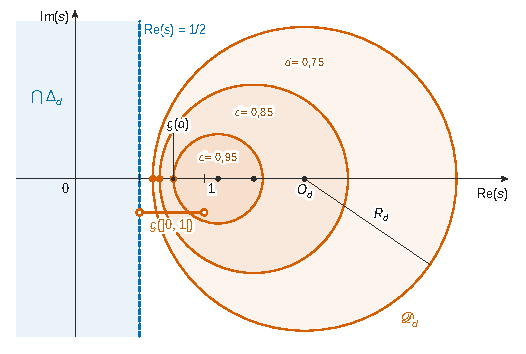
\includegraphics{figures/q14-disques-delta-d.pdf}
\caption*{Figure 1 --- disques 𝒟\_d pour d = 0,95 ; 0,85 ; 0,75, dont le bord
gauche g(d) est strictement entre 1/2 et 1 ; l'intersection des Δ\_d est
le demi-plan fermé Re(s) ⩽ 1/2 (Q12--Q14)}
\end{figure}

\hypertarget{partie-b-uxe9tude-analytique}{%
\section{Partie B --- Étude analytique}\label{partie-b-uxe9tude-analytique}}

\hypertarget{b.i-transformuxe9e-de-mellin-des-fonctions-f_k}{%
\subsection{\texorpdfstring{B.I --- Transformée de Mellin des fonctions \(f_k\)}{B.I --- Transformée de Mellin des fonctions f\_k}}\label{b.i-transformuxe9e-de-mellin-des-fonctions-f_k}}

\hypertarget{q15}{%
\subsection{Q15}\label{q15}}

Pour \(t=\frac1i\), on a \(\lfloor\frac1t\rfloor=i\) et \(\frac1{kt}=\frac ik\).

Si \(1\leqslant i\leqslant k-1\), \(0<\frac ik<1\) donc \(\lfloor\frac ik\rfloor=0\) ; si \(i=k\), \(\lfloor1\rfloor=1\). Ainsi
\equationajustee{\boxed{\begin{aligned}f_k\Bigl(\frac1i\Bigr)&=\frac ik\qquad(1\leqslant i\leqslant k-1),\\f_k\Bigl(\frac1k\Bigr)&=0.\end{aligned}}}

\hypertarget{q16}{%
\subsection{Q16}\label{q16}}

Soit \(t\in\,]0,1]\) et \(m=\lfloor\frac1{kt}\rfloor\in\mathbb N\). Par définition, \(m\leqslant\frac1{kt}<m+1\), donc
\equationajustee{km\leqslant\frac1t<km+k.}
L'entier \(km\) est inférieur ou égal à \(\frac1t\), donc à \(\lfloor\frac1t\rfloor\) (plus grand entier \(\leqslant\frac1t\)).

Et \(\lfloor\frac1t\rfloor\leqslant\frac1t<km+k\) avec des entiers, donc \(\lfloor\frac1t\rfloor\leqslant km+k-1\). Ainsi
\equationajustee{0\leqslant\Bigl\lfloor\frac1t\Bigr\rfloor-km\leqslant k-1,}
et en divisant par \(k\) :
\equationajustee{\boxed{0\leqslant f_k(t)\leqslant\frac{k-1}{k}.}}

\hypertarget{q17}{%
\subsection{Q17}\label{q17}}

D'après Q16, \(kf_k(t)=\lfloor\frac1t\rfloor-k\lfloor\frac1{kt}\rfloor\) est un entier compris entre \(0\) et \(k-1\). Donc
\equationajustee{f_k(]0,1])\subset\Bigl\{\frac jk:0\leqslant j\leqslant k-1\Bigr\}.}
Réciproquement, Q15 montre que \(\frac1k,\dots,\frac{k-1}k\) sont atteints (en \(t=\frac1i\)), et \(0\) aussi (en \(t=\frac1k\)). Donc
\equationajustee{\boxed{f_k\bigl(]0,1]\bigr)=\Bigl\{0,\frac1k,\frac2k,\dots,\frac{k-1}k\Bigr\}.}}

\hypertarget{q18}{%
\subsection{Q18}\label{q18}}

\emph{Lemme des paliers.} Soit \(m\in\mathbb N^*\) et \(t\in\,]\frac1{m+1},\frac1m]\). Alors \(m\leqslant\frac1t<m+1\), donc \(\lfloor\frac1t\rfloor=m\).

Écrivons \(m=kq+r\) (division euclidienne, \(0\leqslant r\leqslant k-1\)). On a
\equationajustee{\frac mk\leqslant\frac1{kt}<\frac{m+1}k=q+\frac{r+1}k\leqslant q+1.}
On en tire \(q\leqslant\frac1{kt}<q+1\), donc \(\lfloor\frac1{kt}\rfloor=q=\lfloor\frac mk\rfloor\). Ainsi
\equationajustee{f_k(t)=\frac mk-\Bigl\lfloor\frac mk\Bigr\rfloor\quad\text{pour } t\in\Bigl]\frac1{m+1},\frac1m\Bigr],}
et \(f_k\) est constante sur chacun de ces intervalles.

\emph{Continuité par morceaux.} Soit \(a\in\,]0,1]\). Le segment \([a,1]\) est recouvert par les intervalles \(]\frac1{m+1},\frac1m]\), \(1\leqslant m\leqslant\lfloor\frac1a\rfloor\), en nombre fini.

Donc \(f_k\) est en escalier sur \([a,1]\). Elle est continue par morceaux sur tout segment de \(]0,1]\), c'est-à-dire sur \(]0,1]\).

\emph{Intégrabilité.} \(|f_k|\leqslant\frac{k-1}k\) (Q16), constante intégrable sur l'intervalle borné \(]0,1]\). \textbf{\(f_k\) est continue par morceaux et intégrable sur \(]0,1]\).}

\begin{figure}[H]
\centering
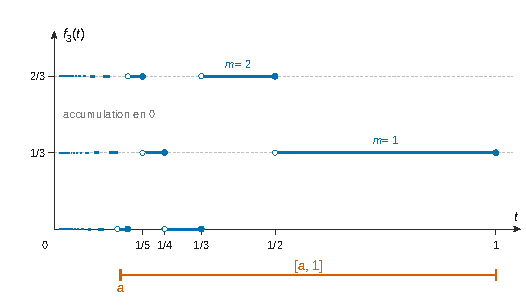
\includegraphics{figures/q18-paliers-f3.pdf}
\caption*{Figure 2 --- paliers de f₃ entre 1/(m+1) (exclu) et 1/m (inclus) :
valeurs 0, 1/3, 2/3, accumulation en 0, nombre fini de paliers sur un
segment d'origine a \textgreater{} 0 (Q18)}
\end{figure}

\hypertarget{q19}{%
\subsection{Q19}\label{q19}}

Soit \(k\geqslant1\) et \(s>1\). La démonstration du lemme des paliers montre que \(t\mapsto\lfloor\frac1{kt}\rfloor\) vaut \(\lfloor\frac mk\rfloor\) sur \(]\frac1{m+1},\frac1m]\).

Elle est donc en escalier sur tout segment de \(]0,1]\), et son produit par \(t\mapsto t^{s-1}\) est continu par morceaux. Comme \(0\leqslant\lfloor u\rfloor\leqslant u\) pour \(u>0\),
\equationajustee{0\leqslant\Bigl\lfloor\frac1{kt}\Bigr\rfloor t^{s-1}\leqslant\frac1k\,t^{s-2}.}
Or \(t\mapsto t^{s-2}=t^{-(2-s)}\) est intégrable sur \(]0,1]\) car \(2-s<1\). Par comparaison de fonctions positives, \textbf{\(\int_0^1\lfloor\frac1{kt}\rfloor t^{s-1}\,\mathrm dt\) converge.}

\hypertarget{q20}{%
\subsection{Q20}\label{q20}}

Sur \(]\frac1{j+1},\frac1j]\), \(\lfloor\frac1t\rfloor=j\). Par Chasles, pour \(N\geqslant1\),
\equationajustee{\int_{1/(N+1)}^1\Bigl\lfloor\frac1t\Bigr\rfloor t^{s-1}\,\mathrm dt=\sum_{j=1}^N j\int_{1/(j+1)}^{1/j}t^{s-1}\,\mathrm dt.}
Le membre de gauche tend vers \(F(s)\) (convergence, Q19 avec \(k=1\)). Donc la série converge et \(F(s)=\sum_{j\geqslant1}j\int_{1/(j+1)}^{1/j}t^{s-1}\,\mathrm dt\).

Ensuite \(\int_{1/(j+1)}^{1/j}t^{s-1}\,\mathrm dt=\frac1s\bigl(j^{-s}-(j+1)^{-s}\bigr)\). Par décalage d'indice,
\equationajustee{\begin{aligned}T_N&=\sum_{j=1}^N j\bigl(j^{-s}-(j+1)^{-s}\bigr)\\&=\sum_{j=1}^N j^{1-s}-\sum_{i=2}^{N+1}(i-1)i^{-s}\\&=\sum_{i=1}^{N+1}\frac1{i^s}-(N+1)^{1-s}\\&\xrightarrow[N\to+\infty]{}\zeta(s)\end{aligned}}
car \(1-s<0\). Donc
\equationajustee{\boxed{\begin{aligned}F(s)&=\sum_{j=1}^{+\infty}j\int_{1/(j+1)}^{1/j}t^{s-1}\,\mathrm dt\\&=\frac1s\,\zeta(s).\end{aligned}}}

\hypertarget{q21}{%
\subsection{Q21}\label{q21}}

Les intégrales \(F(s)\) et \(I_k(s)=\int_0^1\lfloor\frac1{kt}\rfloor t^{s-1}\,\mathrm dt\) convergent (Q19), donc par linéarité
\equationajustee{\int_0^1f_k(t)t^{s-1}\,\mathrm dt=\frac1kF(s)-I_k(s).}
Pour \(t\in\,]\frac1k,1]\), \(\lfloor\frac1{kt}\rfloor=0\) ; pour \(j\geqslant1\), \(\lfloor\frac1{kt}\rfloor=j\iff t\in\,]\frac1{k(j+1)},\allowbreak \frac1{kj}]\). Comme en Q20 (Chasles puis passage à la limite, licite par Q19),
\equationajustee{\begin{aligned}I_k(s)&=\sum_{j=1}^{+\infty}\frac js\Bigl(\frac1{(kj)^s}-\frac1{(k(j+1))^s}\Bigr)\\&=\frac1{k^s}\cdot\frac1s\sum_{j=1}^{+\infty}j\bigl(j^{-s}-(j+1)^{-s}\bigr)\\&=\frac{\zeta(s)}{s\,k^s}.\end{aligned}}
Avec \(F(s)=\frac{\zeta(s)}s\) :
\equationajustee{\boxed{\int_0^1f_k(t)t^{s-1}\,\mathrm dt=\frac1s\Bigl(\frac1k-\frac1{k^s}\Bigr)\zeta(s).}}

\hypertarget{b.ii-prolongement-de-la-fonction-zeta}{%
\subsection{\texorpdfstring{B.II --- Prolongement de la fonction \(\zeta\)}{B.II --- Prolongement de la fonction \textbackslash zeta}}\label{b.ii-prolongement-de-la-fonction-zeta}}

\hypertarget{q22}{%
\subsection{Q22}\label{q22}}

\(h'(t)=-s\,t^{-s-1}\), donc \(|h'(t)|=\frac{s}{t^{s+1}}\), strictement décroissante sur \([k,k+1]\) (\(s+1>0\)). Le maximum est atteint en \(t=k\) :
\equationajustee{\boxed{\max_{[k,k+1]}|h'|=\frac{s}{k^{s+1}}.}}

\hypertarget{q23}{%
\subsection{Q23}\label{q23}}

Notons \(w_k=\int_k^{k+1}\bigl(\frac1{k^s}-\frac1{t^s}\bigr)\mathrm dt\). Pour \(t\in[k,k+1]\), \(t^s\geqslant k^s\) (\(s>0\)), donc l'intégrande est positif et \(w_k\geqslant0\). Par l'inégalité des accroissements finis et Q22,
\equationajustee{0\leqslant\frac1{k^s}-\frac1{t^s}\leqslant\frac{s}{k^{s+1}}(t-k)\leqslant\frac{s}{k^{s+1}},}
d'où \(0\leqslant w_k\leqslant\frac{s}{k^{s+1}}\). La série \(\sum\frac{s}{k^{s+1}}\) converge (\(s+1>1\)), de somme \(s\zeta(s+1)\). Par comparaison, \(\sum w_k\) est une série à termes positifs convergente, et
\equationajustee{\boxed{0\leqslant G(s)\leqslant s\,\zeta(s+1).}}

\begin{figure}[H]
\centering
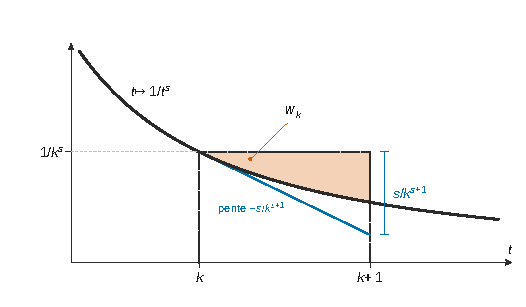
\includegraphics{figures/q23-comparaison-serie-integrale.pdf}
\caption*{Figure 3 --- w\_k est l'aire entre le palier de hauteur 1/kˢ et la
courbe t ↦ 1/tˢ, de k à k+1 ; l'écart vertical est majoré par s/kˢ⁺¹
(Q23)}
\end{figure}

\hypertarget{q24}{%
\subsection{Q24}\label{q24}}

Pour \(s>1\) et \(N\geqslant1\), par Chasles,
\equationajustee{\begin{aligned}\sum_{k=1}^Nw_k&=\sum_{k=1}^N\frac1{k^s}-\int_1^{N+1}\frac{\mathrm dt}{t^s}\\&=\sum_{k=1}^N\frac1{k^s}-\frac{1-(N+1)^{1-s}}{s-1}\\&\xrightarrow[N\to+\infty]{}\zeta(s)-\frac1{s-1}.\end{aligned}}
Donc
\equationajustee{\boxed{\zeta(s)-G(s)=\frac1{s-1}.}}
Soit \(s\in\,]1,2]\). La fonction \(\zeta\) est décroissante sur \(]1,+\infty[\), car chaque \(u\mapsto k^{-u}\) décroît. Avec Q23, on obtient
\equationajustee{0\leqslant G(s)\leqslant s\zeta(s+1)\leqslant2\zeta(2).}
Ainsi \(G\) est bornée au voisinage de \(1^+\) et
\equationajustee{\boxed{\zeta(s)=\frac1{s-1}+O(1)\quad(s\to1^+).}}

\hypertarget{b.iii-intuxe9grale-des-fonctions-f_k}{%
\subsection{\texorpdfstring{B.III --- Intégrale des fonctions \(f_k\)}{B.III --- Intégrale des fonctions f\_k}}\label{b.iii-intuxe9grale-des-fonctions-f_k}}

\hypertarget{q25}{%
\subsection{Q25}\label{q25}}

Pour \(s>1\) et \(t\in\,]0,1]\), \(0<t^{s-1}\leqslant1\), donc \(0\leqslant1-t^{s-1}\leqslant1\) et, par Q16,
\equationajustee{\begin{aligned}\Bigl|\int_0^1f_k(t)t^{s-1}\,\mathrm dt-\int_0^1f_k(t)\,\mathrm dt\Bigr|&\leqslant\frac{k-1}{k}\int_0^1\bigl(1-t^{s-1}\bigr)\mathrm dt\\&=\frac{k-1}{k}\Bigl(1-\frac1s\Bigr)\\&\xrightarrow[s\to1^+]{}0.\end{aligned}}
(Les deux intégrales convergent : \(f_k\) est bornée, continue par morceaux, Q18.) Donc
\equationajustee{\boxed{\int_0^1f_k(t)t^{s-1}\,\mathrm dt\xrightarrow[s\to1^+]{}\int_0^1f_k(t)\,\mathrm dt.}}
(Le théorème de convergence dominée à paramètre réel, avec la domination \(\frac{k-1}k\), conduit au même résultat.)

\hypertarget{q26}{%
\subsection{Q26}\label{q26}}

Pour \(s\in\,]1,2]\), Q21 et Q24 donnent
\equationajustee{\int_0^1f_k(t)t^{s-1}\,\mathrm dt=\frac1s\cdot\frac{\frac1k-\frac1{k^s}}{s-1}+\frac1s\Bigl(\frac1k-\frac1{k^s}\Bigr)G(s).}
Avec \(u=(s-1)\ln k\to0^+\) (\(k\geqslant2\)) :
\equationajustee{\frac{\frac1k-\frac1{k^s}}{s-1}=\frac{\ln k}{k}\cdot\frac{1-e^{-u}}{u}\xrightarrow[s\to1^+]{}\frac{\ln k}{k}.}
Le second terme tend vers \(0\), produit de \(\frac1k-\frac1{k^s}\to0\) par \(G(s)\) bornée (Q24). Donc le membre de gauche tend vers \(\frac{\ln k}{k}\) ; par Q25 il tend aussi vers \(\int_0^1f_k\). Par unicité de la limite,
\equationajustee{\boxed{\int_0^1f_k(t)\,\mathrm dt=\frac{\ln k}{k}.}}

\hypertarget{partie-c-uxe9tude-alguxe9brique-et-guxe9omuxe9trique}{%
\section{Partie C --- Étude algébrique et géométrique}\label{partie-c-uxe9tude-alguxe9brique-et-guxe9omuxe9trique}}

\hypertarget{c.i-une-forme-bilinuxe9aire-symuxe9trique-positive}{%
\subsection{C.I --- Une forme bilinéaire symétrique positive}\label{c.i-une-forme-bilinuxe9aire-symuxe9trique-positive}}

\hypertarget{q27}{%
\subsection{Q27}\label{q27}}

\textbf{a) Vraie.} Si \(|f|\leqslant M\), alors \(0\leqslant f^2\leqslant M^2\), constante intégrable sur l'intervalle borné \(]0,1]\) ; par comparaison, \(\int_0^1f^2\) converge et \(f\in L^2\).

\textbf{b) Fausse.} La fonction \(f:t\mapsto\frac1t\) est continue sur \(]0,1]\), donc dans \(E\). Mais \(\int_\varepsilon^1\frac{\mathrm dt}{t^2}=\frac1\varepsilon-1\to+\infty\) : \(f\notin L^2\). Donc \(L^2\neq E\).

\textbf{c) Fausse.} La fonction \(f:t\mapsto\frac1{\sqrt t}\) est intégrable sur \(]0,1]\), car \(\int_0^1t^{-1/2}\,\mathrm dt=2\). Mais \(f^2=\frac1t\) ne l'est pas (\(\int_\varepsilon^1\frac{\mathrm dt}t=-\ln\varepsilon\to+\infty\)) : \(f\notin L^2\).

\hypertarget{q28}{%
\subsection{Q28}\label{q28}}

De \((|f(t)|-|g(t)|)^2\geqslant0\) on tire \(|f(t)g(t)|\leqslant\frac12\bigl(f(t)^2+g(t)^2\bigr)\). Pour \(f,g\in L^2\), le majorant est intégrable, donc \textbf{\(\int_0^1fg\) converge absolument} par comparaison.

\(L^2\subset E\) contient la fonction nulle. Soit \(f,g\in L^2\) et \(\lambda\in\mathbb R\). Alors \(f+\lambda g\in E\) et
\equationajustee{(f+\lambda g)^2=f^2+2\lambda fg+\lambda^2g^2.}
Les trois intégrales \(\int f^2\), \(\int fg\), \(\int g^2\) convergent. Donc \(\int(f+\lambda g)^2\) converge et \(f+\lambda g\in L^2\).

\textbf{\(L^2\) est un sous-espace vectoriel de \(E\).}

\hypertarget{q29}{%
\subsection{Q29}\label{q29}}

Par Q28, \((f|g)\) est bien défini pour \(f,g\in L^2\). La linéarité de l'intégrale (intégrales convergentes) donne \((f+\lambda g|h)=(f|h)+\lambda(g|h)\).

La symétrie \((f|g)=(g|f)\) est évidente et entraîne la linéarité à droite ; enfin \((f|f)=\int_0^1f^2\geqslant0\). \textbf{C'est une forme bilinéaire symétrique positive.}

Elle n'est pas définie. Soit \(u\) définie par \(u(1)=1\) et \(u(t)=0\) pour \(t\in\,]0,1[\).

Elle est continue par morceaux et bornée, donc dans \(L^2\), non nulle, et \((u|u)=\int_0^1u^2=0\). \textbf{Ce n'est pas un produit scalaire sur \(L^2\).}

\hypertarget{c.ii-un-espace-pruxe9hilbertien-ruxe9el}{%
\subsection{C.II --- Un espace préhilbertien réel}\label{c.ii-un-espace-pruxe9hilbertien-ruxe9el}}

\hypertarget{q30}{%
\subsection{Q30}\label{q30}}

Soit \(t\in\,]\frac12,1]\). Alors \(\frac1t\in[1,2[\) donc \(\lfloor\frac1t\rfloor=1\).

Pour \(k\geqslant2\), \(0<\frac1{kt}<\frac2k\leqslant1\) donc \(\lfloor\frac1{kt}\rfloor=0\). Ainsi \(f_k(t)=\frac1k\), et la relation, évaluée en un tel \(t\) (par exemple \(t=1\)), donne
\equationajustee{\boxed{\sum_{k=2}^n\frac{\lambda_k}{k}=0.}}

\hypertarget{q31}{%
\subsection{Q31}\label{q31}}

Évaluons en \(t=\frac1\ell\) : par Q18 (ou directement), \(f_k(\frac1\ell)=\frac\ell k-\lfloor\frac\ell k\rfloor\).

\begin{itemize}
\tightlist
\item
  Pour \(k>\ell\), \(\lfloor\frac\ell k\rfloor=0\) et le terme vaut \(\lambda_k\frac\ell k\).
\item
  Pour \(k=\ell\), il vaut \(\lambda_\ell(1-1)=0\).
\item
  Pour \(2\leqslant k\leqslant\ell-1\), il reste \(\lambda_k(\frac\ell k-\lfloor\frac\ell k\rfloor)\).
\end{itemize}

D'où
\equationajustee{\boxed{\begin{aligned}{}&\sum_{k=\ell+1}^n\lambda_k\frac\ell k\\&\quad+\sum_{k=2}^{\ell-1}\lambda_k\Bigl(\frac\ell k-\Bigl\lfloor\frac\ell k\Bigr\rfloor\Bigr)=0.\end{aligned}}}

\hypertarget{q32}{%
\subsection{Q32}\label{q32}}

Si \(n=2\), Q30 donne directement \(\lambda_2=0\).

Supposons \(n\geqslant3\). Q31 pour \(\ell=2\) donne \(\sum_{k=3}^n\frac{2\lambda_k}{k}=0\). En retranchant de Q30, \(\frac{\lambda_2}2=0\), donc \textbf{\(\lambda_2=0\)}.

Montrons par récurrence sur \(\ell\in\{2,\dots,n\}\) la propriété \((\mathcal H_\ell)\) :
\equationajustee{\begin{aligned}{}&\lambda_2=\dots=\lambda_{\ell-1}=0\\&\text{et}\ \sum_{k=\ell}^n\frac{\lambda_k}k=0.\end{aligned}}
\((\mathcal H_2)\) est Q30. Supposons \((\mathcal H_\ell)\) vraie avec \(\ell\leqslant n-1\).

Dans Q31 au rang \(\ell\), la seconde somme ne fait intervenir que des \(\lambda_k\) nuls ; il reste \(\sum_{k=\ell+1}^n\frac{\lambda_k}k=0\). La différence avec \((\mathcal H_\ell)\) donne \(\lambda_\ell=0\), d'où \((\mathcal H_{\ell+1})\).

Enfin \((\mathcal H_n)\) donne \(\lambda_2=\dots=\lambda_{n-1}=0\) et \(\frac{\lambda_n}n=0\).

Tous les \(\lambda_k\) sont nuls : \((f_2,\dots,f_n)\) est libre pour tout \(n\). Comme toute sous-famille finie de \((f_k)_{k\geqslant2}\) est incluse dans l'une d'elles,
\equationajustee{\boxed{\text{la famille }(f_k)_{k\geqslant2}\text{ est libre.}}}

\hypertarget{q33}{%
\subsection{Q33}\label{q33}}

Les \(f_k\) et \(\mathbf 1\) sont bornées et continues par morceaux, donc dans \(L^2\) (Q27 a) : \(F\subset L^2\) et la restriction de \((\cdot|\cdot)\) à \(F\) est bilinéaire symétrique positive (Q29). Reste le caractère défini.

Soit \(f=a\mathbf 1+\sum_{k=2}^n\lambda_kf_k\in F\) avec \((f|f)=0\). Par le lemme des paliers (Q18), \(f\) est constante, égale à un réel \(c_m\), sur chaque intervalle \(]\frac1{m+1},\frac1m]\). Par positivité et Chasles,
\equationajustee{\begin{aligned}0\leqslant c_m^2\Bigl(\frac1m-\frac1{m+1}\Bigr)&=\int_{1/(m+1)}^{1/m}f^2\\&\leqslant\int_0^1f^2=0,\end{aligned}}
donc \(c_m=0\) pour tout \(m\geqslant1\). Ces intervalles recouvrent \(]0,1]\), donc \(f=0\). \textbf{\((\cdot|\cdot)\) est un produit scalaire sur \(F\).}

\hypertarget{c.iii-distance-dun-vecteur-uxe0-des-sous-espaces}{%
\subsection{C.III --- Distance d'un vecteur à des sous-espaces}\label{c.iii-distance-dun-vecteur-uxe0-des-sous-espaces}}

\hypertarget{q34}{%
\subsection{Q34}\label{q34}}

\((F,(\cdot|\cdot))\) est préhilbertien (Q33) et \((f_2,\dots,f_n)\) est libre (Q32). Notons \(V_p=\operatorname{Vect}(f_2,\dots,f_p)\). Raisonnons par récurrence sur \(p\).

\emph{\(p=2\).} La condition \(\operatorname{Vect}(e_2)=\operatorname{Vect}(f_2)\) impose \(e_2=\mu f_2\), avec \(\mu\neq0\).

Les conditions \(\|e_2\|=1\) et \((e_2|f_2)=\mu\|f_2\|^2>0\) imposent \(\mu=\frac1{\|f_2\|}\) (\(\|f_2\|>0\) car \(f_2\neq0\)).

Donc \(e_2=\frac{f_2}{\|f_2\|}\), et ce choix convient.

\emph{Hérédité.} Supposons \((e_2,\dots,e_{p-1})\) construite et unique, base orthonormée de \(V_{p-1}\). Posons
\equationajustee{w=f_p-\sum_{j=2}^{p-1}(f_p|e_j)e_j.}
Alors \(w\perp V_{p-1}\), et \(w\neq0\) car \(f_p\notin V_{p-1}\) (liberté). Posons \(e_p=\frac w{\|w\|}\) : la famille \((e_2,\dots,e_p)\) est orthonormale, et
\equationajustee{\begin{aligned}\operatorname{Vect}(e_2,\dots,e_p)&=V_{p-1}+\mathbb Rw\\&=V_{p-1}+\mathbb Rf_p\\&=V_p.\end{aligned}}
Enfin, comme \(f_p-w\in V_{p-1}\),
\equationajustee{(e_p|f_p)=\frac{(w|w+(f_p-w))}{\|w\|}=\|w\|>0.}
Donc \(e_p\) convient.

Unicité : si \(e'_p\) convient, \(e'_p\in V_p\cap V_{p-1}^\perp\). Or \(V_p=V_{p-1}\oplus\mathbb Rw\).

Écrivons \(e'_p=u+\alpha w\) avec \(u\in V_{p-1}\). Alors \(0=(e'_p|u)=\|u\|^2\), donc \(e'_p=\alpha w\).

Puis \(\|e'_p\|=1\) et \((e'_p|f_p)=\alpha\|w\|^2>0\) imposent \(\alpha=\frac1{\|w\|}\), soit \(e'_p=e_p\).

\textbf{Il existe une unique famille orthonormale \((e_k)_{2\leqslant k\leqslant n}\) d'éléments de \(F\subset L^2\) telle que, pour \(2\leqslant p\leqslant n\), \(\operatorname{Vect}(e_2,\allowbreak \dots,\allowbreak e_p)=\operatorname{Vect}(f_2,\allowbreak \dots,\allowbreak f_p)\) et \((e_p|f_p)>0\).}

(Par unicité, la famille obtenue pour \(n+1\) prolonge celle obtenue pour \(n\).)

\hypertarget{q35}{%
\subsection{Q35}\label{q35}}

Soit \(G_n=\operatorname{Vect}(f_2,\allowbreak \dots,\allowbreak f_n)=\operatorname{Vect}(e_2,\allowbreak \dots,\allowbreak e_n)\), de dimension finie, et \(\pi_n\) la projection orthogonale sur \(G_n\). On a
\equationajustee{\pi_n(\mathbf 1)=\sum_{k=2}^n(\mathbf 1|e_k)e_k,}
et \(d_n=\|\mathbf 1-\pi_n(\mathbf 1)\|\) (le projeté réalise la distance). Comme \(\mathbf 1-\pi_n(\mathbf 1)\in G_n^\perp\) et \(\pi_n(\mathbf 1)\in G_n\), Pythagore donne
\equationajustee{\begin{aligned}\|\mathbf 1\|^2&=\|\pi_n(\mathbf 1)\|^2+d_n^2\\&=\sum_{k=2}^n(\mathbf 1|e_k)^2+d_n^2 .\end{aligned}}
Comme \(\|\mathbf 1\|^2=\int_0^11\,\mathrm dt=1\),
\equationajustee{\boxed{d_n^2=1-\sum_{k=2}^n(\mathbf 1|e_k)^2.}}

\begin{figure}[H]
\centering
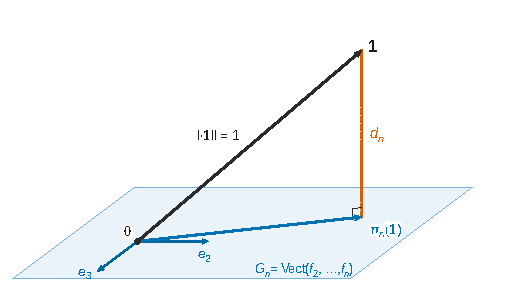
\includegraphics{figures/q35-projection-orthogonale.pdf}
\caption*{Figure 4 --- dₙ est la longueur de la composante de 𝟏 orthogonale à Gₙ ;
Pythagore donne 1 = ‖πₙ(𝟏)‖² + dₙ² (Q35)}
\end{figure}

\hypertarget{q36}{%
\subsection{Q36}\label{q36}}

Comme \(G_n\subset G_{n+1}\),
\equationajustee{d_{n+1}=\inf_{g\in G_{n+1}}\|\mathbf 1-g\|\leqslant\inf_{g\in G_n}\|\mathbf 1-g\|=d_n.}
On peut aussi lire \(d_{n+1}^2=d_n^2-(\mathbf 1|e_{n+1})^2\) sur Q35, la famille \((e_k)\) ne dépendant pas de \(n\).

La suite \((d_n)\) est décroissante et minorée par \(0\) : \textbf{elle converge} (théorème de la limite monotone).

\hypertarget{partie-d-synthuxe8se}{%
\section{Partie D --- Synthèse}\label{partie-d-synthuxe8se}}

\hypertarget{q37}{%
\subsection{Q37}\label{q37}}

Posons \(u=1-\sum_{k=2}^n\lambda_kf_k\) (réelle) et \(v:t\mapsto t^{s-1}\) (complexe).

La fonction \(u\) est continue par morceaux (Q18) et bornée par \(1+\sum|\lambda_k|\) (Q16). Donc \(u^2\) est intégrable sur \(]0,1]\) (Q27 a).

La fonction \(v\) est continue sur \(]0,1]\), et \(|v(t)|^2=t^{2(x-1)}=|t^{2(s-1)}|\) (Q4) est intégrable car \(x>\frac12\) (Q11).

L'inégalité de Cauchy-Schwarz admise s'applique au couple \((u,v)\), avec \(|u|^2=u^2\) :
\equationajustee{\boxed{\Bigl|\int_0^1\Bigl(1-\sum_{k=2}^n\lambda_kf_k(t)\Bigr)t^{s-1}\,\mathrm dt\Bigr|^2\leqslant\int_0^1\Bigl(1-\sum_{k=2}^n\lambda_kf_k(t)\Bigr)^2\mathrm dt\times\int_0^1|t^{2(s-1)}|\,\mathrm dt.}}

\hypertarget{q38}{%
\subsection{Q38}\label{q38}}

Soit \(s\neq1\) avec \(x=\operatorname{Re}(s)>\frac12\) et \(\zeta(s)=0\).

\emph{Intégrale de \(t^{s-1}\).} \(|t^{s-1}|=t^{x-1}\) est intégrable sur \(]0,1]\) (\(x-1>-1\)) et \(t\mapsto\frac{t^s}s\) est une primitive (\(s\neq0\)).

Comme \(|\varepsilon^s|=\varepsilon^x\to0\),
\equationajustee{\begin{aligned}\int_0^1t^{s-1}\,\mathrm dt&=\lim_{\varepsilon\to0^+}\frac{1-\varepsilon^s}{s}\\&=\frac1s.\end{aligned}}

\emph{Intégrales des \(f_k\).} L'égalité de Q21 est admise pour \(s\) complexe de partie réelle \(>0\) distinct de \(1\). Les intégrales sont absolument convergentes car \(|f_k(t)t^{s-1}|\leqslant t^{x-1}\). Pour tout \(k\geqslant2\),
\equationajustee{\int_0^1f_k(t)t^{s-1}\,\mathrm dt=\frac1s\Bigl(\frac1k-\frac1{k^s}\Bigr)\zeta(s)=0.}

\emph{Inégalité.} Par linéarité, pour toute famille réelle \((\lambda_k)\), \(\int_0^1\bigl(1-\sum\lambda_kf_k\bigr)t^{s-1}\,\mathrm dt=\frac1s\), et Q37 avec Q11 donne
\equationajustee{\frac1{|s|^2}\leqslant\Bigl\|\mathbf 1-\sum_{k=2}^n\lambda_kf_k\Bigr\|^2\cdot\frac1{2x-1}.}
Ceci vaut pour toute famille \((\lambda_k)\), en particulier pour celle qui donne \(\sum\lambda_kf_k=\pi_n(\mathbf 1)\), pour laquelle la norme vaut \(d_n\) (Q35). Ainsi
\equationajustee{\boxed{d_n^2|s|^2\geqslant2\operatorname{Re}(s)-1\qquad\text{pour tout }n\geqslant2.}}

\emph{Conclusion.} Si \(d_n\to0\), le passage à la limite donne \(0\geqslant2\operatorname{Re}(s)-1\), soit \(\operatorname{Re}(s)\leqslant\frac12\) : contradiction.

\emph{Lecture géométrique.} L'inégalité dit \(s\in\Delta_{d_n}\). On a \(0<d_n\leqslant d_2=\sqrt{1-\ln2}<1\).

En effet, soit \(L=\operatorname{ppcm}(2,\dots,n)\) : tout élément de \(G_n\) s'annule en \(\frac1L\), donc \(\mathbf 1\notin G_n\) et \(d_n>0\).

De plus \(f_2^2=\frac12f_2\), donc \(\|f_2\|^2=\frac{\ln2}4\) par Q26, et
\equationajustee{\begin{aligned}d_2^2&=1-\frac{(\mathbf 1|f_2)^2}{\|f_2\|^2}\\&=1-\frac{(\ln2/2)^2}{\ln2/4}\\&=1-\ln2.\end{aligned}}
Comme \(\Delta_d\subset\Delta_{d'}\) pour \(d\leqslant d'\), \(d_n\to0\) placerait \(s\) dans \(\bigcap_d\Delta_d=\{\operatorname{Re}\leqslant\frac12\}\) par Q14. Par conséquent :

\textbf{si \(\lim d_n=0\), la fonction \(\zeta\) prolongée ne s'annule en aucun \(s\) tel que \(\operatorname{Re}(s)>\frac12\)} (en \(s=1\), elle n'est pas définie : c'est un pôle).

\end{document}
